\chapter{Background}


In this chapter, we cover the necessary background required for appreciation of this work and the area in general. We begin by describing two of the fundamental building blocks of Semantic Web: 1) Resource Description Format (RDF) that allows a flexible representation of structured information, and 2) the SPARQL query language used to retrieve and manipulate data stored in RDF. Towards the closing, we introduce the Freebase knowledge base---the structured data source that shall be considered primary for the remaining part of this work.


\section[RDF]{Resource Description Format}

Before we dive in head first into the territory of semantic web, we must first understand how it stores data. We start from the ground up by outlining the basic idea of conceptualizing data as a graph---an approach that is many ways contrasted to the relational model assumed by traditional databases.

The fundamental building block of \emph{knowledge graph} (as we shall call it when emphasizing its graph structure), is the notion of an entity. In most applications modelling general-purpose real world information, an entity is something hat has separate and distinct existence and objective or conceptual reality. To make it more concrete, here a few examples of entities:
\begin{itemize}
  \item Indian Institute of Technology, Bombay - an educational institute.
  \item Mumbai - a city
  \item An Evening in Paris - a Bollywood film
  \item Sania Mirza - a person
\end{itemize}

To put it simply, a structured knowledge base captures information about entities. Entities can be related to each other and can have properties (or attributes). The idea of expressing relations between entities is directly borrowed from the notion of Entity-Relationship Model.

Resource Description Framework (RDF) is a framework for representing information about entities in a graph form. It formalizes the notion of entities and relationships between them and the graph thus produced. 

An RDF-triple is a 3-tuple of (subject, predicate, object). While the subject is typically an entity, the object is allowed to be an entity or a non-entity. An RDF object is allowed to be an arbitrary string, which makes it flexible in capturing information such as dates, addresses, and other metadata information that a subject (entity) can be associated with. An RDF predicate is the realization of the concept of a relationship that describes the nature of association between the corresponding subject and object.

\begin{figure}[h!]
  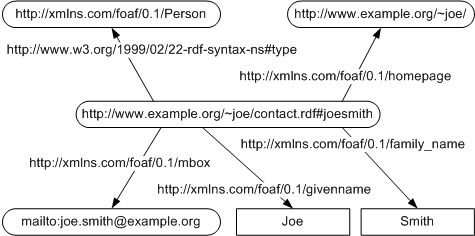
\includegraphics[scale=0.8]{joe-smith-rdf.jpg}
  \caption{An example RDF graph}
  \label{fig:rdfexample}
\end{figure}


Since the RDF evolved around WWW, it encodes the subject, predicate and at times, the object as well, as Uniform Resource Identifiers (URI). An RDF document consists of RDF-triples, typically one triple per line. Figure \ref{fig:rdfexample} illustrates an example RDF graph that the following RDF document represents:

\begin{verbatim}
1: <http://www.example.org/~joe/contact.rdf#joesmith>
      <http://www.w3.org/1999/02/22-rdf-syntax-ns#type>  
      <http://xmlns.com/foaf/0.1/Person>
2: <http://www.example.org/~joe/contact.rdf#joesmith>   
      <http://xmlns.com/foaf/0.1/homepage>
      http://www.example.org/~joe
3: <http://www.example.org/~joe/contact.rdf#joesmith>  
      <http://xmlns.com/foaf/0.1/mbox>
      mailto:joe.smith@example.org
4: <http://www.example.org/~joe/contact.rdf#joesmith>
      <http://xmlns.com/foaf/0.1/givenname>
      Joe
5: <http://www.example.org/~joe/contact.rdf#joesmith>  
      <http://xmlns.com/foaf/0.1/family_name>
      Smith
\end{verbatim}

RDF predicates are represented as labelled arrows that connect an RDF subject (at their tail) to an RDF object (at their head).

Many of the contemporary freely accessible knowledge bases support their distribution in RDF format. While an RDF document is natural way of representing and storing graphs, it is seldom useful in this form. Several RDF databases have emerged that allow loading of RDF documents support APIs that can be used to query and make use of the data. Traditional query languages like SQL are not well suited for querying RDF data, and thus there is a need for query languages and query processing engines that are targeted towards this format. SPARQL is one such query language that has been successful, and we shall now present its brief overview. 


\section[SPARQL]{SPARQL Protocol and RDF Query Language}

SPARQL\cite{prud2008sparql} (recursive acronym for SPARQL Protocol and RDF Query Language) is a semantic query language for RDF databases. SPARQL allows users to write queries against what can loosely be described as ``key-value" data or, more specifically, data that follows the RDF specification of the W3C. 

Though we earlier presented the RDF data model as a graph, it can also be thought of in terms of the SQL relational model as a table with three columns, one each for the subject, the predicate and the object. As we noticed earlier, the data in the object column can be heterogeneous in general, which in contrast with relational databases. The column data type is usually implied by the predicate value or may be specified separately in an ontology. 

As another alternative, all triples belonging to a particular subject may be represented as a single row of the table where the subject is the primary key. A column for each possible predicate may be stored, with the value in a cell storing an RDF object for (row, column) pair of (subject, predicate). However, as is seen in real world datasets, a column could contain multiple values (like the column `family members') for the same row key.

SPARQL provides a full set of analytic query operations such as JOIN, SORT, AGGREGATE for data whose schema is intrinsically part of the data rather than requiring a separate schema definition. Schema information (the ontology) is often provided externally, though, to allow different datasets to be joined in an unambiguous manner. In addition, SPARQL provides specific graph traversal syntax for data that can be thought of as a graph.

\subsection{Example Query}

We shall now illustrate the basic syntax and features of SPARQL using a simple query on the data of Figure \ref{fig:rdfexample}. 

The SPARQL query for retrieving (person, homepage) pairs for all persons in the data, is:
\begin{verbatim}
  PREFIX foaf:   <http://xmlns.com/foaf/0.1/>
  PREFIX w3: <http://www.w3.org/1999/02/22-rdf-syntax-ns>
  FROM foaf:graph
  
  SELECT ?person ?homepage WHERE {
  ?person w3:type foaf:Person,
  ?person foaf:homepage ?homepage
  }
  ORDER BY ?person
\end{verbatim}

Since RDF subjects and predicates are represented as URIs, they tend to have common prefixes. To prevent repetition of these prefixes in the query, the \verb|PERFIX| keyword has been used in the above query. In general, an RDF database might contain multiple RDF graphs. The from keyword allows a user to specify a particular graph to be queried.

The \verb|SELECT| clause asks to specify variables, which are then matched by the triple patterns inside the \verb|WHERE| clause. A triple pattern is simply an RDF triple, whose one or more elements have been replaced by variables. 

It is worth noting that triple patterns allow a natural way of expressing joins without an explicit schema, which makes SPARQL more powerful than storing RDF in a relational schema and running SQL queries on it as was previously discussed.

SPARQL has been implemented in a number of programming languages and graph databases. In particular the Apache Jena Framework and Openlink Virtuoso are widely used implementations of the standard.

\section{Freebase Knowledge Base}

A major prerequisite for the success of Semantic Web is clearly the availability of large amounts of structured data. The effort of building and maintaining comprehensive datasets is largely divided in purpose and content by the organizations supporting these projects. At one end, there are freely accessible knowledge bases such as DBpedia, Wikidata, and Freebase; and at the other there are closed source projects such as Google Knowledge Graph and the Wolfram Knowledgebase. 

For most of our work, we decided to stick to Freebase as our underlying data source. The choice demands us to tweak our approaches slightly to make use of the Freebase schema. Still, the ideas presented are sufficiently general and can be adapted to any of the popular knowledge bases.

Freebase was a large collaborative knowledge base with data curated mainly by its community members. It first appeared in 2007 and was originally developed by the company Metaweb \footnote{en.wikipedia.org/wiki/Metaweb}. Though the project is no longer active, the complete data is available freely through Google Developers\footnote{developers.google.com/freebase}.

Freebase contains tens of millions of topics, thousands of types, and tens of thousands of properties. There are more than a billion facts (loosely, RDF triples) that make up the Freebase graph. The magnitude can be appreciated on the comparison with Wikipedia, which has less than 5 million English articles. 

\subsection{Schema}

The nodes of the Freebase graph are defined using \texttt{/type/object/} and the edges are defined using \texttt{/type/link/}.

Freebase has over 39 million topics about real-world entities like people, places and things. Since Freebase data is represented a graph, these topics correspond to the nodes in the graph. However, not every node is a topic.

Examples of the types of topics found in Freebase:
\begin{itemize}
  \item Physical entities, e.g., Bob Dylan, the Louvre Museum, the Saturn planet, to
  \item Artistic/media creations, e.g., The Dark Knight (film), Hotel California (song), to
  \item Classifications, e.g., noble gas, Chordate, to
  \item Abstract concepts, e.g., love, to
  \item Schools of thoughts or artistic movements, e.g., Impressionism.
\end{itemize}


Any Freebase topic can be seen from different perspectives, For example: Bob Dylan was a song writer, singer, performer, book author, and film actor. In order to capture this multi-faceted nature of many topics, Freebase defines the concept of types. Topics in Freebase can have any number of types assigned to them. The topic about Bob Dylan is assigned several types: the song writer type, the music composer type, the music artist (singer) type, the book author type, etc. Each type carries a different set of properties germane to that type. For example,
\begin{itemize}
\item The music artist type contains a property that lists all the albums that Bob Dylan has produced as well as all the music instruments he was known to play;
\item The book author type contains a property that lists all the books Bob Dylan has written or edited, as well as his writing school of thoughts or movement;
\item The company type contains many property for listing a company's founders, board members, parent company, divisions, employees, products, year-by-year revenue and profit records, etc.
\end{itemize}
Thus, a type can be thought of as a conceptual container of properties that are most commonly needed for describing a particular aspect of information.

We shall describe other features of the Freebase schema, as and when required in the later chapters.